\documentclass[a4paper]{article}

\usepackage[english]{babel}
\usepackage[utf8]{inputenc}
\usepackage[hidelinks]{hyperref}

\usepackage{graphicx}
\graphicspath{ {images/} }

\usepackage{setspace}
\usepackage{pdfpages}
\usepackage{xspace} %Removes space after commands
\usepackage{fancyhdr}
\usepackage{lastpage}
\usepackage{verbatim}
\usepackage{url}

%%% BibTeX %%%
\usepackage{cite}
% JS function to get BibTeX entry from WebAssembly website
\begin{comment}
function BibTeX() {
	let subject = document.title.replace(/ - WebAssembly/, '').replace(' ', '-').toLowerCase();
    return `@misc{website:wasm-${subject}
	author = "The WebAssembly working group",
	title = {{${document.title}}},
	url = "${document.URL}",
	note = {Online; accessed 12 May 2017},
}`;
}
\end{comment}

% source: https://tex.stackexchange.com/a/35044
\makeatletter
\newcommand\footnoteref[1]{\protected@xdef\@thefnmark{\ref{#1}}\@footnotemark}
\makeatother

% Code highlighting
\usepackage{minted}
% Highlight theme
\usemintedstyle{trac}

\pagestyle{fancy}
\fancyhf{}

\lfoot{Page \thepage \hspace{1pt} of \pageref{LastPage}}

\usepackage[margin=0.8in]{geometry}

\title{Bachelor Project Report: Compiling MicroC to WebAssembly}

\begin{document}
%\pagenumbering{gobble} %Remove page numbers
\begin{titlepage}
	\centering
	{\scshape\LARGE IT University of Copenhagen \par}
	\vspace{1cm}
	{\scshape\Large Bachelor Project Report\par}
	\vspace{1.5cm}
	{\huge\bfseries Compiling MicroC to WebAssembly \par}
	\vspace{2cm}
	{
\includegraphics{WebAssemblyLogo} \par}
	\vspace{2cm}
	{\Large\itshape Andreas Bjørn Hassing Nielsen\par}
	abhn@itu.dk\\
	\vspace{2cm}
	{\Large Abstract\par}
	%TODO: Write an awesome abstract.
	{\bfseries This is where the abstract will go.}
	\vfill
% Bottom of the page
	{\large \today\par}
\end{titlepage}

\newpage

\tableofcontents
\newpage


\section{Introduction}
\label{sec:introduction}
The purpose of this project is to build a compiler, also called a translator, from MicroC to WebAssembly, using FsLexYacc\footnote{\label{footnote:fslexyacc-url}http://fsprojects.github.io/FsLexYacc/} and F\#\footnote{http://fsharp.org/}. The learning goals are to develop an understanding of WebAssembly, and to improve my knowledge of compiler design.

MicroC is a C-like language described by Peter Sestoft in the book Programming Language Concepts~\cite{PLC}. The original lexer and parser code can be found at his website\footnote{http://www.itu.dk/people/sestoft/plc/}.

\section{Problem Definition}
\label{sec:problem-definition}
WebAssembly (WASM) is a new up-and-coming binary code format for the user-facing web, designed to work alongside JavaScript as a more portable, size- and load-time-efficient, ahead-of-time-compiled alternative. 

The binary WASM format is not bound to be emitted by JavaScript (asm.js) only, potentially bringing your favourite language to the browser front-end. If a language can compile to a intermediate representation supported by WASM (LLVM IR, for instance), it can be compiled to the binary WASM format. 

The purpose of this project is to shed some light on the unfinished WebAssembly specification. To assist in meeting this goal, a compiler will be designed, that compiles from a simple programming language, MicroC, to a WASM format that can be run in a WASM-enabled browser today (currently requiring Firefox Nightly or Chrome Canary with WASM flags set to enabled\footnote{At the time of writing (May, 2017), setting flags or using a nightly browser version is no longer required. Major browsers now support WASM out of the box: https://lists.w3.org/Archives/Public/public-webassembly/2017Feb/0002.html}).

\subsection{Method}
\label{sec:problem-definition:method}
What follows is the planned activities and sources of information.
\begin{itemize}
	\item Translation of MicroC to the binary WebAssembly format, using FsLexYacc\footnoteref{footnote:fslexyacc-url}, as used in the Programs as Data course (fall 2016).
	\item Course books from Programs as Data (fall 2016) will be used as knowledge base for MicroC to WebAssembly translation:
		\begin{itemize}
			\item Peter Sestoft: Programming Language Concepts. Springer 2012.
			\item Torben Mogensen: Basics of Compiler Design. DIKU 2010. Chapters 2 and 3.
		\end{itemize}
	\item Knowledge of WebAssembly will be gained through the official website (http://webassembly.org/) and links branching out from it.
	\item Creation of prototype: web interface that lets users type MicroC in a window, and see it generate WebAssembly in some human-readable format, either s-expression or linear bytecode. The prototype will also give users the ability to run their code as WebAssembly, given that the browser in use supports it.
	\item Reflection over, either the security behind WebAssembly or the portability of it between browsers and platforms.
\end{itemize}

\noindent If time allows:
\begin{itemize}
	\item Extensions to the MicroC language will be implemented.
	\item Simple optimizations to the generated WebAssembly code.
\end{itemize}
\pagebreak

\subsection{Changes to Method and Problem Definition}
\label{sec:problem-definition:changes}
I realized while coding the compiler that I would have to stop working on it prematurely to get the web back- and frontend working as well. This was an underestimation on my part.

In a meeting with Niels Hallenberg on May 1st we agreed to discard the web part of this project. To make up for the loss I have added a flag (\texttt{-html}) to the compiler which generates a HTML template to go along with the \texttt{.wasm} output. The HTML template makes it easy to test compiled WebAssembly binaries, as you can serve the HTML with a simple HTTP server, see section~\ref{sec:peripherals:testing-wasm},~\nameref{sec:peripherals:testing-wasm}, on how to do that.

\section{Problem Analysis}
\label{sec:problem-analysis}
In this section, the problem will be dissected and analysed. The definition of a compiler is discussed and the WebAssembly specification and binary encoding is scrutinised.

\subsection{Compilers in General}
\label{sec:problem-analysis:compilers}
Before the compiler design is even considered, an important question must be asked and answered: "What is a compiler?".

According to the definition laid out by Mogensen~\cite{BCD}, a compiler is a program that takes the source code of another program as input, usually some higher-level language such as C\#, and compiles it to a lower-level representation, Common Intermediate Language code - in the case of C\#, or binary machine code instructions - in the case of C. There are more low-level representations out in the wild, but these two will be the ones referenced in this report.

Many programs are written in higher-level languages that run within an assisting runtime environment and compiles to a variant of bytecode, with an instruction set specified in the virtual machine of the runtime. When the runtime is started and the program bytecode is passed to it, it performs a just-in-time (JIT) compilation to native machine code using the instruction set of the machine's processor. The .NET CLR and Java's JRE are two such runtimes that both support several higher-level languages, such as C\#, F\#, Java and Scala. Runtime environments often come equipped with integrated memory management in the form of a garbage collector.

Programs written in comparatively lower-level languages, such as C and C++, are usually compiled ahead-of-time (AOT) to native machine code using the instruction set of the compiling machine. One can often configure the compiler to target other operating systems and processor architectures than that of the compiling system. In these lower-level languages, the programmer is often challenged with manually managing dynamic memory.

Note, that nothing stops us from implementing a runtime environment that supports a high-level language, such as C, which can then run code written in that language as a JIT compiled application. The task may be non-trivial.

Then, there is JavaScript, a loosely typed language that runs in browsers. JavaScript is compiled by a JIT compiler at runtime\footnote{This is not always true. Ignition, a newly developed interpreter for V8 (Chrome's JavaScript engine), is used alone or along with JIT compilation, especially on devices where a lower- memory footprint, or battery usage is beneficial (Smartphones, for instance)~\cite{video:thompson-js-perf-v8-and-wasm}.}, which takes the code, turns it into abstract syntax and then to machine code~\cite[p.~13]{slides:lund-v8}. During the execution of a JavaScript program, the JIT compiler will attempt to optimise the generated machine code by making probabilistic assumptions about program behaviour. These assumptions can eventually fail, thus forcing the JIT to throw away optimisations based on falsified claims - this is a cause of non-deterministic execution speed of JavaScript programs. The JIT's that are found in modern browsers make a lot of intelligent optimisations on what is generally referred to as \texttt{warm} and \texttt{hot} code paths\footnote{Warm and hot code describes code paths that are executed regularly and often, respectively.}, thereby greatly increasing performance without sacrificing excessive resources. When a JIT compiler is run on a system with multiple processor cores, it can run in parallel, thereby generating optimisations without blocking the main thread of the program.

\subsubsection{Benefits of AOT Compilation}
\label{sec:problem-analysis:benefits-of-aot}
\textbf{Static Type Checking} When a statically typed language is compiled ahead-of-time, the compiler can complain to the developer before the program hits runtime. For instance, if the developer attempts to assign a char value to a variable that is declared to contain an integer, the compilation will fail. This is useful for producing correct code. JavaScript is a loosely typed language, meaning that type checking happens late, and errors that didn't show during development, can show up in the users browser.\\

\noindent \textbf{Optimisations} While optimisations can be made by both an AOT and JIT compiler, an AOT has all the time a developer has to spare, to optimise. A JIT will need to weigh the potential gain of an optimisation against slowing down the program during the consideration process. This makes an AOT compiler preferred for live and runtime critical systems.

%TODO: add more to AOT benefits?
%TODO: add JIT benefits?

\subsection{History of Web Coding}
\label{sec:problem-analysis:history}
Less than a year ago there was only 1 language that could run natively in all browsers: JavaScript. The web is built around it, and the language has flourished and expanded beyond the land of browsers, in the form of execution environments such as Node.js\footnote{https://nodejs.org/} and native application frameworks such as React Native\footnote{https://facebook.github.io/react-native/} and Electron\footnote{https://electron.atom.io/}.

% TODO: This is rubbish. Redo!
JavaScript is a loosely typed language, which means that types are not checked at compile time, actually, JavaScript is not compiled by the developer at all. The runtime type checks are not too problematic for simple programs running in the browser, but it scales, and with larger applications the checks can be devastating to performance. A JIT compiler in the execution environment will attempt to derive what types variables and functions have in the running program, in order to make some type-check reducing optimisations, but may end up being wrong and discarding them again~\cite{video:thompson-js-perf-v8-and-wasm}. % TODO: is this citation correct?

\subsection{WebAssembly}
\label{sec:problem-analysis:webassembly}
WebAssembly is created to work well together with JavaScript. This is easily deduced from looking at the design of the binary and textual representation of WebAssembly. Code compiled to WASM are turned into modules that can be instantiated from within JavaScript, and WebAssembly modules can selectively describe which components to expose to- and import from JavaScript.

Exported and imported components from and to WASM can be: functions, variables and memory segments. This design allows WASM modules to make use of dependency injections, which can assist in decoupling code and separating implementation concerns.

\subsubsection{Linear Memory}
\label{sec:problem-analysis-webassembly:linear-memory}

\subsubsection{Aligning MicroC and WebAssembly}
\label{sec:problem-analysis-webassembly:aligning}
In this section, some discovered misalignments between MicroC and WebAssembly will be discussed and handled.

\noindent \textbf{The builtin print and println functions.} MicroC has two built-in functions: \texttt{print} and \texttt{println}. They are converted to internal \texttt{printi}, and \texttt{printc} functions, that print an integer and a char respectively. \texttt{println} is simply a call to \texttt{printc} with $10$ as an argument (10 is the new line feed character in ASCII). A few ways on how this could be handled in the conversion to WebAssembly comes to mind:
\begin{itemize}
	\item The functions could be hardcoded as imports in the generated module, thus allowing the compiler to stay MicroC compliant, but forcing the user of the module to supply an implemention of the two functions.
	\item Remove the keywords and functionality from MicroC, and instead implement an \texttt{import} keyword in the compiler, such that function signatures can be specified which could then give the user more power over what kind of functions that must be imported. For instance, \mintinline{c}{import void print(int i);} would require the user of the module to hand an imports object to the module with a print function that takes an integer as argument and returns nothing. This design has a familiar resemblance to prototypes in C.

	A downside to this solution is that it breaks previously working MicroC programs that use the \texttt{print} or \texttt{println} functions.
\end{itemize}

\noindent \textbf{Stack Machine divergences.} The stack machine specified by Peter Sestoft for MicroC and the one specified for WebAssembly are quite different. What follows are some of the major contrasts.

Many instruction codes from the MicroC stack machine do not exist in WebAssembly (\texttt{ldi}, \texttt{sti}, \texttt{dup}, \texttt{swp}, and others). While the opposite is also true, to a great degree, missing instructions in the conversion from a MicroC stack machine to a WebAssembly one is the more problematic direction, as extra instructions in WebAssembly can be ignored.

The instruction code problem leads to the next issue: without \texttt{ldi}, how are variables loaded? It turns out, that WebAssembly does not have the modifiable and globally available stack, as in the MicroC stack machine. In the MicroC stack machine a base- and stack pointer is used to get access to variable adresses and values. In WebAssembly, there are 3 ways of storing and retrieving data: Global variables (using the instruction codes \texttt{set\_global} and \texttt{get\_global}), local variables (\texttt{set\_local} and \texttt{get\_local}) and data stored in linear memory (\texttt{i32.store} and \texttt{i32.load}). Normally, having three ways to do something is a good thing, but only data stored in linear memory can be accessed by address. This can generate some problems, as pointers and arrays are access-by-address.

In the following program, an integer is \texttt{x} is declared and its value set to $5$. Then the address of \texttt{x} is passed to the \texttt{changeInt} function along with the number $42$. At first glance, one could assume that creating a local variable in the \texttt{main} function and using \texttt{get/set\_local} would work, but it wont. Local variables have no addresses, and thus cannot be accessed by functions other than the one that declared it.
\begin{minted}[tabsize=2]{c}
void changeInt(int* i, int to) { *i = to; }
void main() { int x; x = 5; changeInt(&x, 42); }
\end{minted}

Possible solutions to this problem are:
\begin{itemize}
	\item Initially declare all variables defined inside the scope of a function as local, until they are referenced, at which point they are moved from the local environment to linear memory. Any access to the value of a variable inside linear memory variable will happen by dereferencing the address into the linear memory.
	\item An easier to implement version of the proposal above: declare all variables in linear memory, except for function arguments which are special.
\end{itemize}

\section{User Guide and Examples}
\label{sec:user-guide}

\section{Technical Description}
\label{sec:technical}

\section{Testing and Validation}
\label{sec:testing}

\subsection{Known Issues}
\label{sec:testing:known-issues}
What follows are some of the known issues in the compiler:
\begin{itemize}
	\item All function return values MUST be consumed, otherwise the stack will have an incorrect count of elements on the stack at return, and will fail compilation in the browser. A way to solve this would be to ensure that, when the result of a called function is not used, its value is dropped from the stack using the WebAssembly \texttt{drop} instruction.

	Reproducible with:\\
	\mintinline{c}{int iReturn() { return 42; } main() { iReturn(); }}

	\item Array access using the dereferencing operator and addition is not working properly. In\\\nameref{sec:appendix:code:plc-ex2.c} line 27, the compiled program yields incorrect output. Not completely sure why this problem occurs, but I think it has something to do with the offset and relative addresses of variables (which are multiplied by their type width).

	\item Char type variables cannot be dereferenced or used as arrays. This bug exists because I failed to find a way to get the type information of a variable inside \texttt{AccDeref} and \texttt{AccIndex} constructs, so I generalized and used integers for everything. See \nameref{sec:appendix:code:Wasmcomp.fs} lines 228 and 235.

	\item The code that supports compilation of variable access (the \texttt{varAccess} function in \nameref{sec:appendix:code:Wasmcomp.fs}, lines 202 to 242) is a mess and is not very readable. Not really a bug, but probably the reason behind some.  Unfortunately, due to time constraints, I didn't get to clean it up.

	\item In the original MicroC compiler (written by Peter Sestoft), out of scope variables bleed into other scopes. A test, see \nameref{sec:appendix:code:test-scope.c}, revealed this problem. This issue does not exist in MicroWac by keeping track of the depth of variables, and declaring them as being outside of a scope as soon as the scope ends.
\end{itemize}

\section{Peripheral Programs and Tooling}
\label{sec:peripherals}
This section describes the use of peripheral programs and tooling that assist in, compiling the compiler, or exposing the generated code from compiled MicroC programs.

\subsection{Inspecting WASM Binaries}
\label{sec:peripherals:inspecting-wasm}
To inspect WebAssembly binaries (and to ensure correctness) a few hexviewers were used: HxD\footnote{https://mh-nexus.de/en/hxd/} on Windows, and https://hexed.it/ on OS X and Linux.

\subsection{Lexer and Parser Generator}
\label{sec:peripherals:lexpargen}
Generating the parser and lexer is done by the tool: FsLexYacc. Unfortunately, FsLexYacc does not know if it needs to recompile, as changes are not tracked, thus it will always recompiles if it is added to the build process. Once the generator had delayed work enough times, a small solution was thought up, see appendix section~\ref{sec:appendix:code:pre-build-lexpar-comp},~\nameref{sec:appendix:code:pre-build-lexpar-comp}.

The pre-build scripts (a \texttt{.sh} version for *nix and a \texttt{.ps1} version for Windows) generates- and checks the hashes of the lexer and parser files. If the hash has changed from the cached version, it regenerates the lexer and parser. It was first written in PowerShell, then converted to Bash.

Under the hood the scripts use Gits' \texttt{hash-object} command, in order to stay OS agnostic.

\subsection{Testing \texttt{.wasm} output}
\label{sec:peripherals:testing-wasm}
Due to time constraints, the compiler is not directly exposed to a web environment\footnote{See section~\ref{sec:problem-definition:changes},~\nameref{sec:problem-definition:changes}.} This severely reduces the simplicity of using the compiler, so a helping flag was introduced in the compiler: \texttt{-html}. If this flag is set while compiling, the compiler will generate a HTML file that loads the \texttt{.wasm} file.

A piece of JavaScript code in the HTML file uses the \texttt{fetch} API found in browsers. This API is not allowed via the \texttt{file://} protocol, thus requiring the file to be served with the \texttt{http://} protocol. It is, however, easy to run a webserver that exposes files on \texttt{http://localhost:<port>} with either Python (2 or 3) or Node.js.

To start a web server in the local directory with Node installed, first install \texttt{http-server} globally with: \verb$npm install -g http-server$. Once installed, the server can be started with the command \texttt{http-server} in the directory containing the HTML file(s).

Node may not be readily available, in which case maybe Python is. To start a web server with Python2, run the command \texttt{python -m SimpleHTTPServer}, and for Python3, run the command \texttt{python -m http.server}, no installation is required for either command.

\subsection{Prototyping in F\#}
\label{sec:peripherals:prototyping}
Prototyping different solutions with F\# is extremely easy. This fact was abused rigorously throughout the development process of the compiler. There was rarely a need to compile the compiler, and changes could be tested quickly with the following command:\\
\texttt{fsi -r \textasciitilde/fsharp/FsLexYacc.Runtime.dll Absyn.fs CPar.fs CLex.fs Parse.fs WasmMachine.fs WasmComp.fs}

This command opens up F\# interactive with the compiler loaded. To use the compiler within interactive type in: \texttt{open MicroWac;;} and start using the functions. By not including the \texttt{.fsi} files in the command, access is obtained to all functions, even those not exposed by the signature files - a neat trick.

\section{Future Extensions}
\label{sec:extensions}

\subsection{Compiler Optimisations}
\label{sec:extensions:optimisations}
Humans (should) write readable and maintainable code. A computer only cares about operations, and each operation costs some $x$ energy and time. The compiler can perform optimisations to reduce the amount of operations a program needs for some logic to be completed, this machine code reduction positively influences the compiled program, by reducing the energy consumed by a processor running it, and increasing the performance.

\textbf{Peephole optimisation} is a simple technique that consumes few resources and little time. The cause of this is that peephole optimisations only require knowledge of a few close operations in order to apply reductions.

\begin{figure}[H]
	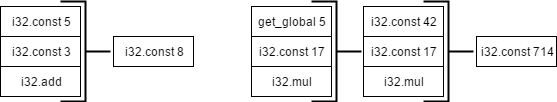
\includegraphics[width=0.65\textwidth]{PeepholeOptimisationIllustrations}
	\centering
	\caption{The applied optimisation to the left stack is simple: adding two constants can be reduced to the result of the addition. The optimisation on the right hand side is more complex: suppose we have a global at position 5 that is immutable and contains the value 42. We can convert the get-call to the value of the variable, as it will never change, which leads to an operation sequence that resembles the one on the left hand side - which, then again, can be can be optimised even further.}
\end{figure}

In a forward compiler, optimising with peephole style optimisations can be added as a pass in the backend compiler, such that when the instruction code is generated, the compiler will run through it again, this time attempting to apply optimisations which attempts to reduce and remove code. For instance, if a function in a program adds two constants together and returns the result, an optimising compiler will reduce the expression to the result of the addition operation, and simply return that: \mintinline{c}{return 7+14; => return 21;}. The logic has not been tampered with, but the function is now 3 operations cheaper\footnote{One for each of the stack reads (reading 7 and 14) and then one for the resulting write operation.}. A more elaborate example can be found below.

\begin{figure}[H]
	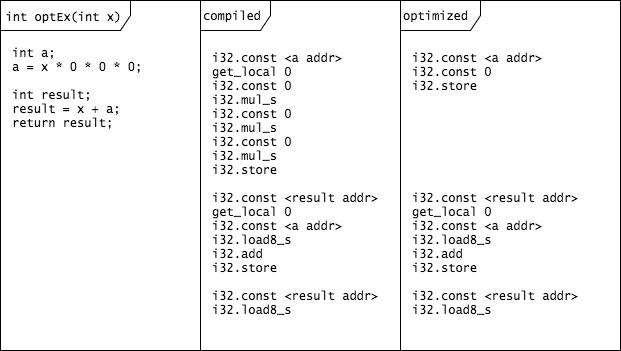
\includegraphics[width=0.75\textwidth]{PeepholeOptimisation}
	\centering
	\caption{A simple function \texttt{optEx} multiplies the input argument with $0$ a few times and then returns the result of an addition. To the right of the function are the compiled and optimised versions of the code in WebAssembly stack machine code.}
\label{fig:peephole-optimisation}
\end{figure}
As can be seen in figure~\ref{fig:peephole-optimisation}, only the multiplication expressions are simplified. While peephole optimising, the compiler will not know if it can discard \texttt{a} entirely, as it could be referenced later, and the compiler does not know the value of \texttt{x}, nor what \texttt{a} contains anymore (we can see that it is equal to $0$, but our brains collect a lot of state regarding the program at hand, which allows us to deduce this), therefore, nothing can be optimised at the end of the function. Running a more complex and stateful optimisation technique could detect more redundant code, but such an optimisation is more resource- and time consuming.

Peephole optimisations fall short when more elaborate optimisations are needed. For instance, if you have many small functions you may want to inline them where used. If we reuse the example from above, with the add function, simply adding the result to the stack rather than calling the function each place is fewer operations, thus inlining would yield a benefit. During peephole optimisation, you won't have information regarding the environment, thus you won’t know what the function that is being called will do, and will not know if inlining is legal.

\section{Conclusion}
\label{sec:conclusion}

\section{References}
\label{sec:references}
\begingroup
\renewcommand{\section}[2]{}%
\bibliographystyle{plain}
\bibliography{Bibliography}{}
\endgroup

\newpage
\section{Appendix}
\label{sec:appendix}

\subsection{Code}
\label{sec:appendix:code}
The full source code can be found in the \texttt{.zip}-file that contained this report. If you only have the report in PDF format, see https://github.com/AndreasHassing/microc-to-webassembly.

\subsubsection{micro-wac/pre-build-lexpar-comp.\{sh$|$ps1\}}
\label{sec:appendix:code:pre-build-lexpar-comp}
\textbf{PowerShell Version}
\inputminted[breaklines,tabsize=2,linenos]{powershell}{../micro-wac/pre-build-lexpar-comp.ps1}

\newpage
\noindent\textbf{Bash Version}
\inputminted[breaklines,tabsize=2,linenos]{bash}{../micro-wac/pre-build-lexpar-comp.sh}

\newpage
\subsubsection{micro-wac/Wasmcomp.fs}
\label{sec:appendix:code:Wasmcomp.fs}
\inputminted[breaklines,tabsize=2,linenos]{fsharp}{../micro-wac/Wasmcomp.fs}

\newpage
\subsubsection{micro-wac/test/scope.c}
\label{sec:appendix:code:test-scope.c}
\inputminted[breaklines,tabsize=2,linenos]{c}{../micro-wac/test/scope.c}

\newpage
\subsubsection{micro-wac/test/plc/ex2.c}
\label{sec:appendix:code:plc-ex2.c}
\inputminted[breaklines,tabsize=2,linenos]{c}{../micro-wac/test/plc/ex2.c}

\end{document}
